\chapter{The Boundary of the Manifold: Blowup, Turbulence and Steady Flows}
\label{ch:boundary}

\section{Where the derivation stops}

The strong derivations of Chapters~\ref{ch:kinetic} and~\ref{ch:hydro} are valid for as long as the limiting equations have smooth solutions. In three dimensions nobody knows how long that is. The weak derivation of Golse and Saint Raymond~\cite{golsesaintraymond2004} needs no smoothness and ends in Leray solutions of the limiting fluid equations, but Leray solutions are not known to be unique, so it does not select a solution once smoothness may fail. The solution manifold of Chapter~\ref{ch:nsinference} therefore has a boundary: the set of initial conditions whose trajectories cease to be smooth, if it is not empty, and the regime of fully developed turbulence, in which solutions are smooth in principle but so rough in practice that only statistical descriptions are meaningful.

\section{Leray and the regularity problem}

In 1934 Jean Leray~\cite{leray1934} proved that for every initial velocity of finite energy in $\R^3$ there is a global weak solution of the Navier Stokes equations satisfying the energy inequality
\[
\frac12\|u(t)\|_{L^2}^2+\nu\int_0^t\|\nabla u(s)\|_{L^2}^2\dd s\leq\frac12\|u(0)\|_{L^2}^2.
\]
He called such solutions turbulent solutions, conjecturing that singularities might be the mathematical origin of turbulence, and he proposed a mechanism: a self similar solution
\[
u(t,x) = \frac{1}{\sqrt{2a(T^*-t)}}\,U\Big(\frac{x}{\sqrt{2a(T^*-t)}}\Big)
\]
whose profile $U$ solves a stationary elliptic system. Ne\v{c}as, R\r{u}\v{z}i\v{c}ka and \v{S}ver\'ak~\cite{necas1996} proved in 1996 that no nontrivial profile in $L^3(\R^3)$ exists, and Tsai~\cite{tsai1998} extended this to profiles in $L^q(\R^3)$ for every $q>3$ and to self similar solutions that satisfy the local energy estimates. Escauriaza, Seregin and \v{S}ver\'ak~\cite{ess2003} showed in 2003 that a solution of the unforced equations bounded in $L^\infty_tL^3_x$ cannot blow up, so any singularity must make the critical $L^3$ norm unbounded.

The partial regularity theorem of Caffarelli, Kohn and Nirenberg~\cite{ckn1982} shows that for suitable weak solutions the singular set has one dimensional parabolic Hausdorff measure zero, hence parabolic Hausdorff dimension at most one: singularities, if they exist, are rare in space time. The Beale, Kato and Majda criterion~\cite{bkm1984}, proved for Euler and valid also for Navier Stokes, shows that a smooth solution on $[0,T^*)$ blows up at $T^*$ if and only if, for the vorticity $\omega=\operatorname{curl}u$,
\[
\int_0^{T^*}\|\omega(t)\|_{L^\infty}\dd t = \infty.
\]

Tao~\cite{tao2016} constructed finite time blowup for an averaged version of the Navier Stokes equations that obeys the same energy identity, showing that energy methods alone cannot prove regularity. Buckmaster and Vicol~\cite{buckmastervicol2019} proved nonuniqueness of weak solutions with finite energy by convex integration; these solutions are not required to satisfy the energy inequality, so they are not Leray solutions. Albritton, Bru\'e and Colombo~\cite{abc2022} proved nonuniqueness of Leray solutions with a suitably chosen forcing. For the Euler equations, Elgindi~\cite{elgindi2021} proved finite time singularity formation for $C^{1,\alpha}$ velocity fields for some small $\alpha>0$, and Chen and Hou~\cite{chenhou2022,chenhou2025} gave a computer assisted proof of stable, nearly self similar blowup of the axisymmetric equations for smooth data of finite energy in the presence of a boundary, confirming the scenario found numerically by Luo and Hou~\cite{luohou2014}. The regularity question for smooth data in $\R^3$ without boundary remains open.

\section{Blowup as a parameter}\label{sec:blowup_param}

From the inferential point of view, the blowup time is a functional of the initial condition, possibly infinite, and its posterior is a well defined object. Self similar or type I blowup predicts $\|\omega(t)\|_{L^\infty}\approx c/(T^*-t)$ near the singular time, the rate that makes the Beale Kato Majda integral diverge logarithmically. Hence the reciprocal $y(t) = 1/\|\omega(t)\|_{L^\infty}$ is approximately linear in $t$ and vanishes at $T^*$.

\begin{proposition}[Posterior for the blowup time]
\label{prop:blowup_time}
Suppose $y_j = a+bt_j+\xi_j$ for $j = 1,\dots,m$, with $\xi_j\sim N(0,\sigma^2)$ independent and $\sigma$ known. Let $X$ be the $m\times2$ matrix with rows $(1,t_j)$, let $(c_{\cdot\cdot}) = (X^\top X)^{-1}$, and let $(\hat a,\hat b)$ be the least squares estimate. Take the prior flat on $\R^2$ and set $T^* = -a/b$ if $b<0$ and $T^* = +\infty$ if $b\geq0$. The posterior of $(a,b)$ is Gaussian with mean $(\hat a,\hat b)$ and covariance $\sigma^2(X^\top X)^{-1}$, the posterior probability of no blowup is
\[
\P(T^* = +\infty\mid\text{data}) = \P(b\geq0\mid\text{data}) = \Phi\Big(\frac{\hat b}{\sigma\sqrt{c_{bb}}}\Big),
\]
where $\Phi$ is the standard normal distribution function, and on $\{b<0\}$ the posterior of $T^*$ is that of $-a/b$, a ratio of correlated Gaussians. The Fieller set~\cite{fieller1954}
\[
F_\gamma = \Big\{T:\frac{(\hat a+\hat bT)^2}{\sigma^2(c_{aa}+2c_{ab}T+c_{bb}T^2)}\leq z_{1-\gamma/2}^2\Big\},
\]
with $z_{1-\gamma/2} = \Phi^{-1}(1-\gamma/2)$, contains the zero $-a/b$ of the line with sampling probability exactly $1-\gamma$, for every $(a,b)$ with $b\neq0$, and it is bounded if and only if $\hat b^2>z_{1-\gamma/2}^2\sigma^2c_{bb}$.
\end{proposition}

\begin{proof}
The posterior is the standard result for the Gaussian linear model with a flat prior, and the marginal of $b$ is $N(\hat b,\sigma^2c_{bb})$, which gives the probability of no blowup. For fixed $T$ put $q(T) = c_{aa}+2c_{ab}T+c_{bb}T^2$, which is positive because $(c_{\cdot\cdot})$ is positive definite. Under the sampling law $\hat a+\hat bT$ is $N(a+bT,\sigma^2q(T))$, so at $T = -a/b$, when $b\neq0$, the statistic $(\hat a+\hat bT)^2/(\sigma^2q(T))$ has the $\chi^2_1$ law and does not exceed $z_{1-\gamma/2}^2$ with probability $1-\gamma$. This is the coverage. The set $F_\gamma$ is $\{Q\leq0\}$ for the quadratic $Q(T) = (\hat a+\hat bT)^2-z_{1-\gamma/2}^2\sigma^2q(T)$. If its leading coefficient $\hat b^2-z_{1-\gamma/2}^2\sigma^2c_{bb}$ is positive, then $\hat b\neq0$ and $Q(-\hat a/\hat b) = -z_{1-\gamma/2}^2\sigma^2q(-\hat a/\hat b)<0$, so $F_\gamma$ is a bounded interval. If the leading coefficient is negative, then $Q<0$ outside a bounded set. If it is zero, then $\hat b\neq0$, $Q$ is affine, and the same value shows that $\{Q\leq0\}$ is not empty, so it is a half line or $\R$. In the last two cases $F_\gamma$ is unbounded.
\end{proof}

The set $F_\gamma$ has exact coverage as a confidence set. As a posterior statement it is conservative, but only when the fitted line is close to zero. Whitening the posterior shows that the posterior probability that $-a/b$ lies in $F_\gamma$ depends on the data only through $r = \|X(\hat a,\hat b)^\top\|/\sigma$, the norm of the fitted values in units of $\sigma$. It equals $1$ for $r\leq z_{1-\gamma/2}$ and tends to $1-\gamma$ as $r\to\infty$; for $\gamma = 0.05$ numerical integration gives $0.982$, $0.954$ and $0.9505$ at $r = 2$, $2.5$ and $3$. Once the fitted line is more than a few noise standard deviations from zero, $F_\gamma$ is therefore a credible set of level $1-\gamma$ to good approximation, whether or not the slope is well determined.

The proposition shows that the evidence for a finite singular time in a computed solution is a statistical statement, the boundedness of a Fieller set, and that the natural summary of a simulation at fixed resolution is a posterior distribution over $T^*$ that places mass on $+\infty$ when the slope is not well determined. For $\hat b<0$ the two statements agree: $F_\gamma$ is bounded exactly when $\P(b\geq0\mid\text{data})<\gamma/2$. The model treats the error of the solver as independent Gaussian noise of constant variance on $y$, and this is its main limitation. The discretization error is deterministic, it is correlated in time, and it grows as the solution approaches the singular time. A fuller treatment puts a prior on the exponent as well, $\|\omega\|_\infty\approx c(T^*-t)^{-\theta}$, whose posterior distinguishes type I from type II scenarios, and replaces the independent noise by a model of the discretization error.

For forced equations blowup has been proved in several settings. For every $\beta<\frac12$, C\'ordoba and Mart\'inez Zoroa~\cite{cordoba2023} constructed solutions of the forced three dimensional Euler equations on $\R^3$, with a force bounded in $C^{1,\beta}\cap L^2$ uniformly in time, for which $\int_0^t\|\nabla u\|_{L^\infty}\dd s\to\infty$ as $t$ approaches a finite time. They also showed~\cite{cordoba2024} that the two dimensional incompressible porous media equation with a compactly supported source, smooth in space uniformly in time, has a smooth finite energy solution that becomes singular at a finite time. With Zheng they proved~\cite{cordoba2026} that the forced hypodissipative Navier Stokes equations on $\R^3$ with positive viscosity have solutions of finite energy, smooth in space before a finite time and with $\int_0^t\|\nabla u\|_{L^\infty}\dd s\to\infty$ as $t$ approaches it, for a force in $L^1_tC^{1,\beta}_x\cap L^\infty_tL^2_x$ with some $\beta>0$ and dissipation exponents $0\leq\alpha<(11-4\sqrt7)/9\approx0.046$ in the notation of Section~\ref{sec:hypodiss}. Alp\"oge, Buckmaster and Coiculescu~\cite{alpoge2026} proved finite time blowup for the porous media equation on the torus $\T^2$ with a force that is smooth in space and time, and announce analogous results of Alp\"oge and Buckmaster, with proofs in preparation, for the forced two dimensional inviscid Boussinesq equations and for the forced three dimensional Euler equations among axisymmetric solutions with swirl. None of these results concerns the Navier Stokes equations themselves, $\alpha = 1$.

For forced problems the forcing is itself an unknown function, and the question of whether a smooth forcing can drive a given flow to blowup is an inverse problem. One possible prior favors sparsity, a few localized forcing modes rather than many. The horseshoe prior of Carvalho, Polson and Scott~\cite{carvalho2010}, treated in Chapter~\ref{ch:mixtures}, shrinks small coefficients strongly and leaves large ones nearly unshrunk, which is the behavior wanted here. We have not tested it on this problem and offer it as a proposal.

\section{Hypodissipation and the Mat\'ern connection}\label{sec:hypodiss}

Replacing $\nu\Delta$ by $-\nu(-\Delta)^\alpha$ gives the hypodissipative ($\alpha<1$) or hyperdissipative ($\alpha>1$) Navier Stokes equations. J.\,L.~Lions~\cite{lions1969} showed in 1969 that for $\alpha\geq5/4$ in three dimensions smooth solutions exist globally: the dissipation then controls the nonlinearity at the critical scaling, since the energy is critical when $\alpha = 5/4$. Tao~\cite{tao2009} improved this by a logarithm. For $\alpha<5/4$ and no forcing, whether smooth solutions exist globally is open, as it is for the classical case $\alpha = 1$; with forcing, blowup has been proved for small $\alpha$, as described in Section~\ref{sec:blowup_param}.

The operator $(\kappa^2-\Delta)^\alpha$ is the precision operator of the Mat\'ern Gaussian field of Chapter~\ref{ch:mixtures}. Consider the linear hypodissipative Stokes system on the torus, driven by space time white noise projected onto solenoidal fields. Its stationary law is Gaussian and supported on solenoidal fields, with spectral density proportional to $|k|^{-2\alpha}$ times the projection onto the plane orthogonal to $k$, a Mat\'ern law with $\kappa = 0$, and in three dimensions its shell summed energy spectrum is proportional to $k^{2-2\alpha}$. In this linear model the dissipation exponent of the dynamics and the smoothness parameter of the stationary statistics are the same parameter, and a measured spectrum carries information about $\alpha$. The gamma mixture representation of the Mat\'ern class suggests that a posterior for $\alpha$ can be computed by data augmentation, which we have not implemented. The inference does not extend to the nonlinear equations. In the inertial range the argument of Section~\ref{sec:k41} gives the spectrum $k^{-5/3}$ for every $\alpha$, since it uses only the dissipation rate and the wavenumber, and the linear model would read this spectrum as $\alpha = 11/6$, which lies outside the range $\alpha<5/4$ where regularity is open.

\section{Turbulence: Kolmogorov 1941}\label{sec:k41}

Richardson's cascade picture of 1922~\cite{richardson1922}, in which large eddies break into smaller ones until viscosity dissipates them, was made quantitative by Kolmogorov in 1941~\cite{kolmogorov1941a,kolmogorov1941b}. Assume that at high Reynolds number the statistics of velocity increments $\delta u(\ell) = u(x+\ell)-u(x)$ at scales $\ell$ in an inertial range, far from both the forcing scale and the viscous scale, are homogeneous, isotropic and determined by the mean energy dissipation rate per unit mass $\varepsilon$ alone. Dimensional analysis then gives the structure functions $S_p(\ell) = \E|\delta u(\ell)|^p\propto(\varepsilon\ell)^{p/3}$ and the energy spectrum
\[
E(k) = C_K\,\varepsilon^{2/3}k^{-5/3}.
\]
Kolmogorov derived an exact relation for the third order longitudinal structure function, and from it the four fifths law. It is a statement of physics and not a theorem about solutions of the Navier Stokes equations, because its hypotheses are those of the physical picture. The flow is statistically stationary, homogeneous and isotropic, it is maintained by a forcing at a scale $L_f$, and the mean dissipation $\varepsilon = \nu\E|\nabla u|^2$, which equals the mean power injected by the forcing, remains positive as $\nu\to0$. Whether solutions of the Navier Stokes equations behave in this way is the question of anomalous dissipation, which is open (Section~\ref{sec:onsager_conjecture}).

For the increments of such a flow, the Navier Stokes equations with forcing $f$ give the K\'arm\'an Howarth Monin balance
\[
\nabla_\ell\cdot\E\big[|\delta u|^2\delta u\big] = 2\nu\Delta_\ell\E|\delta u|^2-4\varepsilon+2\E[\delta u\cdot\delta f],
\]
where $\delta f$ is the increment of the forcing. For $\ell$ much smaller than $L_f$ the last term is negligible. Isotropy and incompressibility reduce the balance to a relation between the longitudinal structure functions $S_2^\parallel(\ell) = \E[(\delta u_\parallel)^2]$ and $S_3^\parallel(\ell) = \E[(\delta u_\parallel)^3]$, where $\delta u_\parallel$ is the component of the increment along the separation,
\begin{equation}\label{eq:kh_exact}
S_3^\parallel(\ell) = -\frac45\varepsilon\ell+6\nu\,\partial_\ell S_2^\parallel(\ell).
\end{equation}
The balance and its isotropic reduction are derived in Frisch~\cite{frisch1995}. In the inertial range $\eta\ll\ell\ll L_f$, where $\eta = (\nu^3/\varepsilon)^{1/4}$ is the Kolmogorov scale, $S_2^\parallel\propto(\varepsilon\ell)^{2/3}$, so the viscous term is smaller than the first term by a factor of order $(\eta/\ell)^{4/3}$, and what remains is Kolmogorov's four fifths law
\begin{equation}\label{eq:fourfifths}
\E\big[(\delta u_\parallel(\ell))^3\big] = -\frac45\varepsilon\ell.
\end{equation}
The law is one of the few exact results about three dimensional turbulence. The four thirds law $\E[\delta u_\parallel|\delta u|^2] = -\frac43\varepsilon\ell$ and the K\'arm\'an Howarth equation are others~\cite{frisch1995}.

Rigorous versions need hypotheses that the physical statement does not make. Duchon and Robert~\cite{duchonrobert2000} showed that a weak solution of the Euler equations in $L^3$ on the torus satisfies a local energy balance with a defect distribution $D$. When the solution is the strong $L^3$ limit of Leray solutions $u^\nu$ of the Navier Stokes equations, $D$ is the distributional limit of $\nu|\nabla u^\nu|^2$ plus the nonnegative defect of $u^\nu$ itself, so $D\geq0$. If $\ell^{-1}\delta u_\parallel|\delta u|^2$, averaged over the direction of the separation, converges in the sense of distributions as $\ell\to0$, then $D$ is $-\frac34$ times the limit: this is a local four thirds law. Eyink~\cite{eyink2003} showed that under the same kind of assumption $\ell^{-1}(\delta u_\parallel)^3$, averaged over directions, converges to $-\frac45D$, which is the four fifths law in the same local sense, and that the mixed moment with one longitudinal and two transverse increments gives the four fifteenths law. Bedrossian, Coti Zelati, Punshon Smith and Weber~\cite{bcpw2019} proved an averaged four fifths law, averaged over space and over the direction of the separation, for stationary martingale solutions of the Navier Stokes equations on $\T^3$ forced by noise that is white in time and colored in space. Their only assumption on the solutions is weak anomalous dissipation, $\nu\E\|u\|_{L^2}^2\to0$ as $\nu\to0$, and the law holds uniformly for $\ell_D(\nu)\leq\ell\leq\ell_I$ in the limit $\nu\to0$ followed by $\ell_I\to0$, where $\ell_D(\nu)\to0$. Whether solutions satisfying this assumption exist is open.

Kolmogorov~\cite{kolmogorov1962} and Obukhov~\cite{obukhov1962}, in the same issue of the \emph{Journal of Fluid Mechanics}, revised the theory in 1962 to account for intermittency, the fluctuation of the local dissipation rate, and proposed that the dissipation averaged over a ball of radius $\ell$ is lognormal with a variance growing like $\log(L/\ell)$. The refined theory predicts structure function exponents $\zeta_p$ that deviate from $p/3$, as observed. It is a curious coincidence, though a natural one from the point of view of Chapter~\ref{ch:mixtures}, that Thorin's original motivation~\cite{thorin1977} for generalized Gamma convolutions was to prove that the lognormal law is infinitely divisible: the dissipation field of K62 is a multiplicative cascade, an infinite product of independent factors, and its logarithm is an infinite sum. Multifractal models such as that of She and Leveque~\cite{sheleveque1994}, $\zeta_p = \frac p9+2\big(1-(\frac23)^{p/3}\big)$, are log infinitely divisible cascades in this sense.

\section{Onsager's conjecture}\label{sec:onsager_conjecture}

Onsager~\cite{onsager1949} observed in 1949 that a constant energy flux $\varepsilon$ through scale $\ell$, of order $|\delta u|^3/\ell$, requires $|\delta u|\sim(\varepsilon\ell)^{1/3}$, the scaling of the four fifths law. The velocity field of turbulence at zero viscosity therefore cannot be more regular than H\"older continuous of exponent one third, since otherwise the flux would vanish as $\ell\to0$ and energy would be conserved. An unpublished note of 1945 to C.\,C.~Lin contains an identity analogous to the four fifths law, and Eyink and Sreenivasan~\cite{eyinksreenivasan2006} infer that it was the basis of the claim. Onsager conjectured that weak solutions of the Euler equations conserve energy if their H\"older exponent exceeds one third, and that dissipative solutions exist with any exponent below one third.

\begin{theorem}[Constantin, E and Titi; Isett]
\label{thm:onsager}
Let $T>0$ and consider weak solutions of the incompressible Euler equations on $[0,T]\times\T^3$, in the sense of distributions. If $u\in L^3(0,T;C^{0,\beta}(\T^3))$ with $\beta>\frac13$, then $\int_{\T^3}|u(x,t)|^2\dd x$ is constant for almost every $t$. For every $\beta<\frac13$ there is a weak solution $u\in C([0,T];C^{0,\beta}(\T^3))$ whose energy $\int_{\T^3}|u(x,t)|^2\dd x$ is not constant in $t$.
\end{theorem}

We quote both halves without proof. The first half was proved by Constantin, E and Titi~\cite{cet1994} in 1994 by a commutator estimate on mollified equations, and Bardos and Titi~\cite{bardostiti2018} proved it in a bounded domain $\Omega$ with $C^2$ boundary, for solutions with $u\cdot n = 0$ on $\partial\Omega$ that lie in $L^3(0,T;C^{0,\beta}(\overline\Omega))$ with $\beta>\frac13$. The second half was proved by Isett in 2018~\cite{isett2018}, completing a program of convex integration begun by De Lellis and Sz\'ekelyhidi~\cite{delellisszekelyhidi2009}. Buckmaster, De Lellis, Sz\'ekelyhidi and Vicol~\cite{bdsv2019} showed that for every $\beta<\frac13$ and every smooth positive energy profile $e(t)$ there is a weak solution in $C^\beta([0,T]\times\T^3)$ with energy $e(t)$, so that a decreasing profile gives strictly dissipative solutions. Onsager's threshold is now a theorem, and anomalous dissipation is mathematically possible. Whether it is the mechanism of real turbulence, that is, whether vanishing viscosity limits of Navier Stokes solutions dissipate energy at a positive rate, remains open.

From the inferential standpoint, the dissipation rate $\varepsilon$, the Kolmogorov constant $C_K$, and the exponents $\zeta_p$ are parameters of a statistical model for velocity increments, and their posterior distributions given measured increments are the natural objects. The four fifths law gives a moment condition for $\varepsilon$; the higher structure functions inform the intermittency parameters. A Bayesian analysis of turbulence data is therefore a mixture model problem, and the scale mixture machinery of Chapter~\ref{ch:mixtures} applies directly. Conditionally on the local dissipation the increments cannot be Gaussian, since a centered Gaussian has zero third moment. The model of Section~\ref{sec:infer_dissipation} instead writes the increment as $(\varepsilon_\ell\ell)^{1/3}Z$ with $Z$ skewed, and the local dissipation $\varepsilon_\ell$ is lognormal or log infinitely divisible.

\section{Steady flows and flow MRI}

At the other end of the spectrum from turbulence lie steady laminar flows,
\[
u\cdot\nabla u+\nabla p = \nu\Delta u,\qquad\nabla\cdot u = 0\quad\text{in }\Omega,\qquad u = g\ \text{on }\partial\Omega.
\]
In medical and engineering applications the domain $\Omega$, the boundary data $g$ and the viscosity are partly unknown, and the velocity is measured, noisily and at limited resolution, by magnetic resonance velocimetry. Kontogiannis, Elgersma, Sederman and Juniper~\cite{kontogiannis2025} formulated this as a Bayesian inverse problem in which the unknowns are the inlet velocity, the outlet conditions, the shape of the boundary, represented implicitly by a viscous signed distance function, and the viscosity, and computed the maximum a posteriori estimate by an adjoint based iteration. A quasi Newton (BFGS) approximation of the inverse Hessian, which is the posterior covariance of the Laplace approximation, accelerates the iteration. The reconstructed velocity field satisfies the Navier Stokes equations by construction, and quantities that are difficult to measure, such as the pressure and the wall shear stress, follow from the reconstruction. The method was tested on magnetic resonance data of a steady flow through a physical model of an aortic arch. Estimating the posterior uncertainty from the approximate covariance is left to future work in that paper.

In the language of this book, the boundary data play the role of the initial condition, the solution manifold is the set of steady solutions indexed by boundary data and shape, and the reconstruction is projection onto that manifold. Two extensions are natural, and neither has been carried out for flow MRI. The first uses the adjoint computation as a summary statistic, in the manner of Chapter~\ref{ch:manifold}. The gradient of the data misfit at a fixed reference state costs one adjoint solve per dataset, once the forward solve at the reference state is done, whereas the maximum a posteriori estimate needs a forward and an adjoint solve at every step of the optimization. A generator trained on simulations to map this statistic to posterior draws could capture non Gaussian features of the posterior that the Laplace approximation misses. The second is that the shape uncertainty, which is non Gaussian because shapes form a manifold, could be represented by transport maps of the kind discussed in Chapter~\ref{ch:gbc}.

\section{The boundary as a modeling frontier}

The three regimes of this chapter differ in their mathematics but share an inferential structure. In each, the deterministic solution manifold is either incompletely understood or practically inaccessible at the relevant resolution, and statistical modeling enters not as a convenience but as a necessity. The sixth problem, read inferentially, asks for a calculus in which such statistical descriptions are derived from, or at least made consistent with, the underlying equations. The Bayesian framework supplies the calculus, and the remaining chapters develop its computational and statistical mechanical side.

\section{Burgers' equation: an exactly solvable model}

The one dimensional Burgers equation
\[
\partial_tu+u\,\partial_xu = \nu\,\partial_x^2u
\]
shares the quadratic nonlinearity and the dissipation of Navier Stokes but none of its geometric complexity, and it can be solved exactly. Hopf~\cite{hopf1950} and Cole~\cite{cole1951} observed in 1950 and 1951 that the substitution $u = -2\nu\,\partial_x\log\phi$ transforms it into the heat equation $\partial_t\phi = \nu\,\partial_x^2\phi$. With $u_0 = U_0'$, the solution is
\[
u(t,x) = \frac{\int\frac{x-y}{t}\exp\big(-\frac{(x-y)^2}{4\nu t}-\frac{U_0(y)}{2\nu}\big)\dd y}{\int\exp\big(-\frac{(x-y)^2}{4\nu t}-\frac{U_0(y)}{2\nu}\big)\dd y}.
\]
The formula has a Bayesian reading that is exact. Regard $y$ as an unknown initial position, give it the improper prior proportional to $e^{-U_0(y)/2\nu}$, and observe the position $x$ of a Brownian particle with diffusion coefficient $\nu$ at time $t$. Then $u(t,x) = \E[(x-Y)/t\mid x]$, the posterior mean of the average velocity of the particle given its endpoint. The Hopf Cole transform is the Feynman Kac formula of Chapter~\ref{ch:quantum} for the heat equation.

As $\nu\to0$, Laplace's method replaces the posterior mean by the posterior mode, the minimizer of $\frac{(x-y)^2}{2t}+U_0(y)$, which is the Hopf Lax formula of the inviscid equation. Where the minimizer jumps, the solution has a shock. Figure~\ref{fig:burgers} shows the solution for three viscosities: as $\nu$ decreases, the profile steepens into a shock. The energy dissipation rate $\nu\int(\partial_xu)^2\dd x$ does not vanish as $\nu\to0$ once a shock forms: the gradient grows like $1/\nu$ over a layer of width $\nu$, so the dissipation converges to a positive limit determined by the jump. This is anomalous dissipation in its simplest form, the one dimensional caricature of Onsager's mechanism, and it is rigorous. In the posterior language, a shock is a point at which the posterior over initial positions becomes bimodal: two different initial points are equally good explanations of the observed position, and the limit selects between them discontinuously.

\begin{figure}[t]
\centering
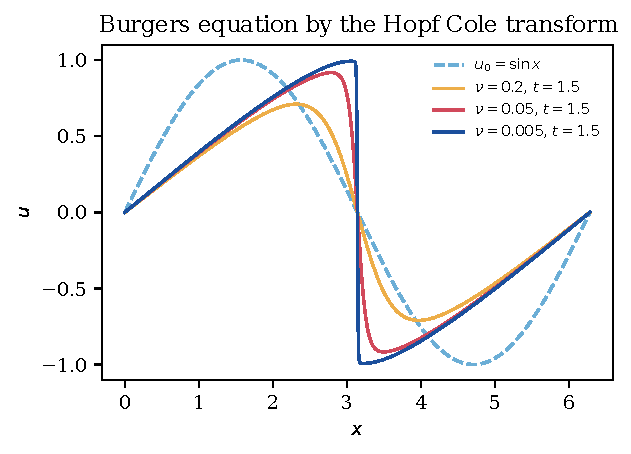
\includegraphics[width=0.92\textwidth]{burgers}
\caption{Solutions of the Burgers equation at $t=1.5$ for $\nu=0.2$, $0.05$ and $0.005$, computed by quadrature of the Hopf Cole formula from the initial condition $u_0=\sin x$, which is also drawn. The shock at $x=\pi$ forms in the inviscid limit.}
\label{fig:burgers}
\end{figure}

Burgers turbulence, the statistical theory of Burgers equation with random initial data or forcing, was developed by Sinai~\cite{sinai1992}, by E, Khanin, Mazel and Sinai~\cite{ekms2000}, and by others. For forcing that is periodic in space and white in time the inviscid equation has a unique invariant measure~\cite{ekms2000}, described through one sided minimizers of the action, and the structure functions scale as $S_p(\ell)\propto\ell$ for $p\geq1$ as $\ell\to0$~\cite{evandeneijnden2000}, a pure bifractal intermittency caused by the shocks. The exponents are therefore known exactly, which makes the model a test case for statistical methods that estimate scaling exponents from data.

\section{Inferring the dissipation rate}\label{sec:infer_dissipation}

The four fifths law gives a moment equation for $\varepsilon$, but in practice the inertial range is short and the third order structure function is noisy. A Bayesian model combines all scales. Let $\delta u_\parallel(\ell_j)$ be measured longitudinal increments at separations $\ell_1<\dots<\ell_J$. Conditionally on a local dissipation $\varepsilon_\ell$ at scale $\ell$, the K62 hypothesis gives increments of the form $\delta u\approx(\varepsilon_\ell\ell)^{1/3}Z$ with $Z$ a skewed variable independent of $\varepsilon_\ell$ and $\E Z^3 = -\frac45$, and $\log\varepsilon_\ell$ Gaussian with mean $\log\varepsilon-\frac{\mu}{2}\log(L/\ell)$ and variance $\mu\log(L/\ell)$, where $\mu$ is the intermittency coefficient. The mean and variance give $\E\varepsilon_\ell = \varepsilon$, so that $\E(\delta u)^3 = \ell\,\E\varepsilon_\ell\,\E Z^3 = -\frac45\varepsilon\ell$, which is the four fifths law. The model is a scale mixture in the sense of Chapter~\ref{ch:mixtures}, with lognormal mixing, and data augmentation over the latent $\varepsilon_\ell$ gives a posterior for $(\varepsilon,\mu,L)$ that can be sampled by Markov chain Monte Carlo. For a general law of $Z$ the lognormal mixing is not conjugate and the sampler needs Metropolis steps. We have not carried out the computation. The posterior of $\mu$ would be the statistical quantity behind the debate over the departure of structure function exponents from $p/3$, and the posterior of $\varepsilon$ given finite resolution data would quantify how sharply the anomalous dissipation hypothesis can be tested.

\section*{Exercises}
\begin{enumerate}
\item Verify that the Hopf Cole substitution transforms the Burgers equation into the heat equation.
\item Write the stationary elliptic system satisfied by a Leray self similar profile $U$.
\item Derive Fieller's interval for the ratio of two jointly Gaussian quantities with known covariance.
\item Using the scaling $u_\lambda(t,x) = \lambda^{2\alpha-1}u(\lambda^{2\alpha}t,\lambda x)$, show that the energy is critical for the hypodissipative equations in three dimensions exactly when $\alpha = 5/4$.
\item For the inviscid Burgers equation with $u_0 = \sin x$, show that the shock forms at time one.
\end{enumerate}


\section*{Notes}

Robinson, Rodrigo and Sadowski~\cite{robinson2016} treat the three dimensional regularity problem in detail. Frisch's \emph{Turbulence: The Legacy of A.\,N.~Kolmogorov}~\cite{frisch1995} is the standard account of K41, K62 and multifractals. De Lellis and Sz\'ekelyhidi~\cite{delellisszekelyhidi2017} survey convex integration and Onsager's conjecture, and Eyink and Sreenivasan~\cite{eyinksreenivasan2006} review Onsager's work on turbulence, published and unpublished.
